\section{The Human Knowledge Residual: a construct to measure}\label{sec:residual}

The research program has one target quantity that no one has measured yet: the \emph{Human
Knowledge Residual} (HKR). This section defines it, separates it from nearby quantities, and states
how it would be measured. Nothing here is a finding; the HKR may be small, unmeasurable or
unpredictable.

\evlit{} Cognitive task analysis (CTA) measures omission against other experts
(\cref{sec:problem}), and reporting-bias research shows that writers omit what is obvious to them
\parencite{gordon2013reporting}. Neither measures the gap between \emph{a body of text} and
\emph{what practitioners use}. \evint{} The term is not established. Its nearest analogues are
unseen-item estimation \parencite{chao1987estimating,chao2012coverage}, also used for undetected
software defects \parencite{briand2000comprehensive}, recall of knowledge bases
\parencite{razniewski2024completeness}, and knowledge loss after developer turnover
\parencite{rigby2016quantifying}.

\subsection{Operational definition}

\begin{evhypbox}
  Fix a task scope $D$ and an evidence base $E$: a specified set of World~A (and optionally
  World~B) sources, found by a fixed search protocol and frozen at a date $t$. The \emph{Human
  Knowledge Residual} $\mathrm{HKR}(D, E, t)$ is the set of knowledge items that meet two
  conditions. (1)~Competent practitioners of $D$ \emph{demonstrably use} the item. It appears in
  elicitation or a performance trace, and a second practitioner, a trace, or an artifact outside
  $E$ corroborates it (such as a log that shows the item in use without stating it). (2)~$E$
  \emph{does not contain} the item: no span in $E$ states it, as judged under a fixed codebook by
  blind coders or by a matcher that meets the adoption rule ($\kappa \geq 0.70$). We hypothesize
  that this set is not empty where practice matters and that it concentrates in certain knowledge
  types (cues, decision rules, checks, rationale). We also hypothesize that its location can be
  predicted from $E$ alone better than by cheap baselines.
\end{evhypbox}

The definition is \emph{relative}: a new source can shrink the HKR. It does not claim that
knowledge is tacit \enquote{in itself}; Collins' relational tacit knowledge, unsaid for contingent
reasons, is included by design \parencite{collins2010tacit}. It requires \emph{use, not report}: an
item one expert says but no one performs or corroborates does not count. And it concerns the
\emph{evidence base, not a model}: model output without a located span is labeled
\code{synthetic_extrapolation} and is not part of $E$ (\cref{sec:evidence-model}).

\paragraph{Counting.} Let $R$ be the items the reconstruction extracted from $E$ and $H$ the
validated human items. Following \repo{REORIENTATION.md} §14.1, the observed residual share is
$\mathrm{Res}_{\mathrm{obs}} = |H \setminus R| \,/\, |H \cup R_{\mathrm{valid}}|$, where
$R_{\mathrm{valid}}$ is the part of $R$ that humans judge valid, reported per knowledge type and per
area. The converse $R \setminus H$ (valid items experts did not say) is reported beside it, never as
error. \evint{} $H \setminus R$ is an upper bound on the residual, not the residual. It splits into
$H \setminus E$, the residual, and $(H \cap E) \setminus R$, the reconstruction misses: items $E$
states that the pipeline did not extract. An area is \emph{residual-present} if it holds at least one
validated, important item of $H \setminus E$; an area with such items only in
$(H \cap E) \setminus R$ is \emph{miss-present} and is scored separately. Residual-present is the
label the gap map is scored against. Telling the two apart needs each item checked against the
frozen corpus: the \enquote{is it really unsaid?} decision the PoC's absence check did not make
reliably (\cref{sec:n3}). So the residual cannot be measured more reliably than absence can be
judged. Absence has two parts, retrieval (does the searched pool hold the stating span?) and
judgment (does a span state the item?); the closure study (V1) measures both, before any grant.

\begin{figure}[tbp]
  \centering
  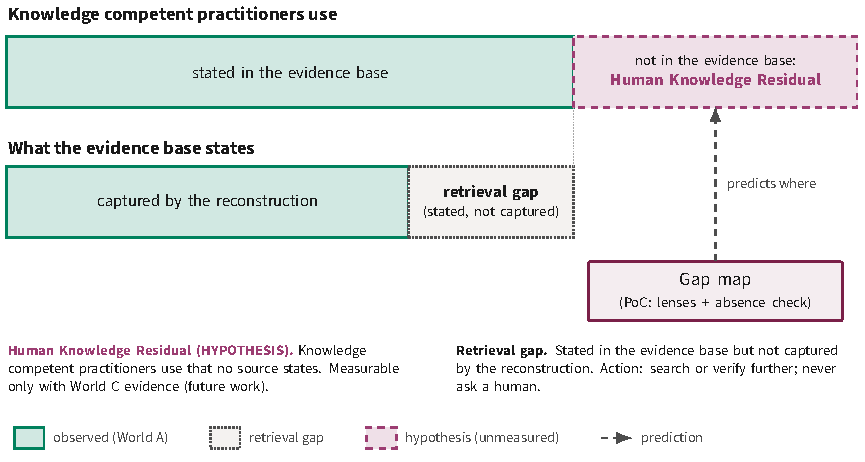
\includegraphics{figures/pdf/fig12_residual.pdf}
  \caption[The Human Knowledge Residual]{What is the Human Knowledge Residual, and how would it
    be measured? The reconstruction $R$ is drawn from a frozen evidence base $E$; validated human
    items $H$ come from elicitation and traces (World~C). The residual is the part of $H$ that $E$
    does not state; items that $E$ states but $R$ missed are reconstruction misses. Thinness is a
    property of $R$ alone. The gap map predicts, from $R$ only and before any human is asked,
    where the residual lies. Dashed elements are not built.}
  \label{fig:residual}
\end{figure}

\paragraph{What each study measures in place of the HKR.} \evint{} Only the prospective study (V5)
measures the construct as defined, and V5 decides H2. The others measure named proxies. In the
pooled CTA gold study (V2), published gold lists stand in for $H$: their items were elicited and
published, not re-validated by use. V2 therefore screens; it does not decide. The
developer-departure study (V3) measures realized knowledge loss after a departure (rationale-seeking
issues and defect-fix commits), predicted from coverage of code artifacts. That is a different
construct, so V3 tests a separate organizational hypothesis (H-OSS) and can neither support nor
refute H2 (\cref{sec:validation}).

\paragraph{Thinness is not the residual.} Three quantities must not be blurred. \emph{Thinness} is
a property of the ledger $R$ alone (source density, independent sources, retrieval gaps,
\code{UNKNOWN} slots, cross-run agreement); the PoC computed it for three ledgers. The \emph{HKR} is
a relation of $H$ to $E$, not yet measured. The \emph{gap-map prediction} is an area score,
$P(\mathrm{residual\ present} \mid \mathrm{area})$, labeled \code{inferred}; none is built yet.
On PLC the gap-map score tracks source density closely (\cref{sec:n3}). \evint{} An area can be thin
because retrieval was poor or because the knowledge is unwritten; only human evidence tells the two
apart. Hence density and area size are headline baselines in every test.

\subsection{How the residual would be measured}

\evfut{} The protocol reuses the registered rules of \repo{REORIENTATION.md} §14 and §18.
\begin{enumerate}[noitemsep]
  \item Freeze and hash-commit $E$, $R$, the area partition, the gap map and its area score before
    any human data exist.
  \item Elicit with a channel matched to the knowledge type: CDM-style retrospective probes for
    episode-specific cues \parencite{klein1989critical}, observation or traces for automated
    procedure, contrasting cases for perceptual cues. At least one arm stays blind to $R$.
  \item Segment transcripts into items at a grain fixed in a codebook.
  \item Validate each item by a second expert, a trace or an artifact outside $E$. Other experts
    rate importance later, blind to how the area was chosen.
  \item Match each item against $R$ and the frozen corpus, by blind coders or by a model matcher
    that meets the adoption rule (\cref{sec:validation}).
  \item Count per area and type.
  \item Estimate unseen items from text occasions only after a known-truth check against published
    gold (V4). Text occasions share authors and pretraining, so they underestimate stably
    \parencite{chao1987estimating,briand2000comprehensive}.
\end{enumerate}
A residual of zero is never reported. What makes this hard (incomplete gold, method-dependent
elicitation, matcher error, a moving evidence base) is treated with the program's threats
(\cref{sec:validation}).

\begin{evobsbox}
  The accounting types exist and refuse these shortcuts. \code{ResidualAccount} computes
  $H \setminus R$, $R \setminus H$, recall by type and $\mathrm{Res}_{\mathrm{obs}}$. It raises
  \code{ResidualNotMeasurable} when an item of $R \setminus H$ lacks a human validity judgment, and it
  rejects a non-human validity rater and a model matcher from the generator's family. No estimator
  is implemented, nothing produces the declared \code{GapMapPrediction} type, and no World~C data
  exist.\footnote{\repo{residual/src/residual/residual.py}.}
\end{evobsbox}

\paragraph{Why it would matter.} \evhyp{} If the HKR is non-trivial and measurable, each validated item of $H \setminus E$ can be
stored with its domain, knowledge type, revealing channel and pre-elicitation gap-map score
(\repo{REORIENTATION.md} §14.5). Across domains this \emph{residual corpus} would calibrate gap
maps, give CTA research a measure of omission relative to text, supply validated hidden steps for
instruction (\cref{sec:education}), and show which organizational units depend on people
(\cref{sec:organizations}). \evint{} A small residual would also be informative: there, expert time
belongs to verification, not elicitation.
